\documentclass[14pt]{article}

\usepackage{amssymb}
\usepackage{mathtools}
\usepackage{tikz}
\usepackage{wasysym}

\let\oldemptyset\emptyset{}
\let\emptyset\varnothing{}

\begin{document}

\section*{Chapter 2}

\subsection*{Exercise 2.1.1.2}
$\mathcal{P}(A) = \emptyset, \{1\}, \{2\}, \{3\}, \{1,2\}, \{1,3\}, \{2,3\}, \{1,2,3\}$

\subsection*{Exercise 2.1.1.3}
\paragraph{a.}
A function $PR \to RG$.
\paragraph{b.}
Yes, there are probably many many-to-one connection points.

\subsection*{Exercise 2.1.2.5}
\paragraph{a.}
$2 \mapsto 4$
\paragraph{b.}
$0 \mapsto 0$
\paragraph{c.}
Not applicable; $-2 \not\in \mathbb{N}$.
\paragraph{d.}
$5 \mapsto 25$
\paragraph{e.}
The symbol $\to$ associates the domain and codomain, while $\mapsto$
associates a particular member of the domain to a particular member of
the codomain.

\subsection*{Exercise 2.1.2.6}
$\operatorname{im}(f) = \{y_1, y_2, y_4\}$

\subsection*{Exercise 2.1.2.8}
$f(A) = \{0,1,4,9\}$

\subsection*{Exercise 2.1.2.10}
$f \circ x \colon \{\smiley\} \to Y$ and $\smiley \mapsto f(x)$.

\subsection*{Exercise 2.1.2.12}
\paragraph{a.}
$2^5 = 32$
\paragraph{b.}
$5^2 = 25$

\subsection*{Exercise 2.1.2.13}
\paragraph{a.}
Take $A := \{\smiley\}$.  (e.g. $A := $
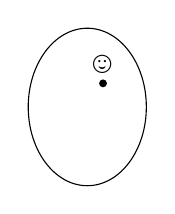
\begin{tikzpicture}
  \draw (0,0) ellipse [x radius = 0.75, y radius = 1];
  \fill (0.2,0.3) circle [radius=0.05] node[anchor=south]{\smiley};
\end{tikzpicture}
, $X := $
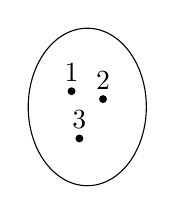
\begin{tikzpicture}
  \draw (0,0) ellipse [x radius = 0.75, y radius = 1];
  \fill (-0.2,0.2) circle [radius=0.05] node[anchor=south]{1};
  \fill (0.2,0.1) circle [radius=0.05] node[anchor=south]{2};
  \fill (-0.1,-0.4) circle [radius=0.05] node[anchor=south]{3};
\end{tikzpicture}
)
\paragraph{b.}
$B := \emptyset$.  (e.g. $B := $
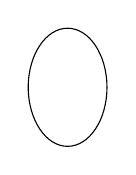
\begin{tikzpicture}
    \draw (0,0) ellipse [x radius = 0.50, y radius = 0.75];
\end{tikzpicture}
)

\subsection*{Exercise 2.1.2.17}

\end{document}
